\subsection{Architektura aplikacji}

\subsubsection{Wzorce projektowe}

\paragraph{Wzorzec "Budowniczy"}
Tworzenie obiektu mapy postanowiłem rozwiązać za pomocą wzorca Buildera - 
specjalna klasa MapBuilder udostępnia metody, które pozwalają inkrementacyjnie 
dodawać coraz to nowe szczegóły do mapy, a następnie zwrócić gotowy widok, 
który został już przetłumaczony do HTML~\cprotect\footnote{%
    W aktualnym kształcie aplikacji narzucony jest zwracany typ \verb|string|, 
    ale w przyszłości może zostać zaimplementowana obsługa natywnych widoków,
    przez co typ zostanie odpowiednio zmieniony.}.

\paragraph{Wzorzec MVVM}
W aplikacji starałem się korzystać ze wzorca projektowego MVVM~\ref{mvvmSubsection} - 
wprowadziłem podział na odpowiednio:
\begin{itemize}
    \item Pliki znaczników - strona\verb|.xaml| wraz z code-behind 
    (kodu związanego bezpośrednio z danym widokiem) - strona\verb|.xaml.cs|
    \item ViewModel, przygotowany dla każdego widoku - strona\verb|ViewModel.cs|
    \item Modele, przechowywane w specjalnym folderze \verb|Models| oraz ujęte w odrębnej przestrzeni nazw
\end{itemize}

Zamysł polega na uniemożliwieniu bezpośrednich interakcji danych 
modelowych z widokami, a poprzez ViewModele. Takie podejście umożliwia bezpieczną zmianę 
widoków, bez zastanawiania się czy wpłyną one na zachowanie ViewModelu lub co gorsza wprost na dane.
Na rysunku  widzimy skrótowy podział rozwiązania na klasy, pogrupowany 
zgodnie z ich przeznaczeniem oraz najważniejszą relacją z klasami sąsiadującymi.
\subsubsection{Podział na projekty}
\begin{figure}[!h]
    \centering
    \frame{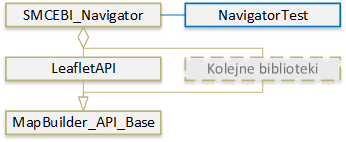
\includegraphics[width=0.7\textwidth]{projectDiagram.png}}
    \caption{Podział rozwiązania na projekty}
    \label{img:projectDiagram}
\end{figure}

\begin{figure}[ht]
    \centering
    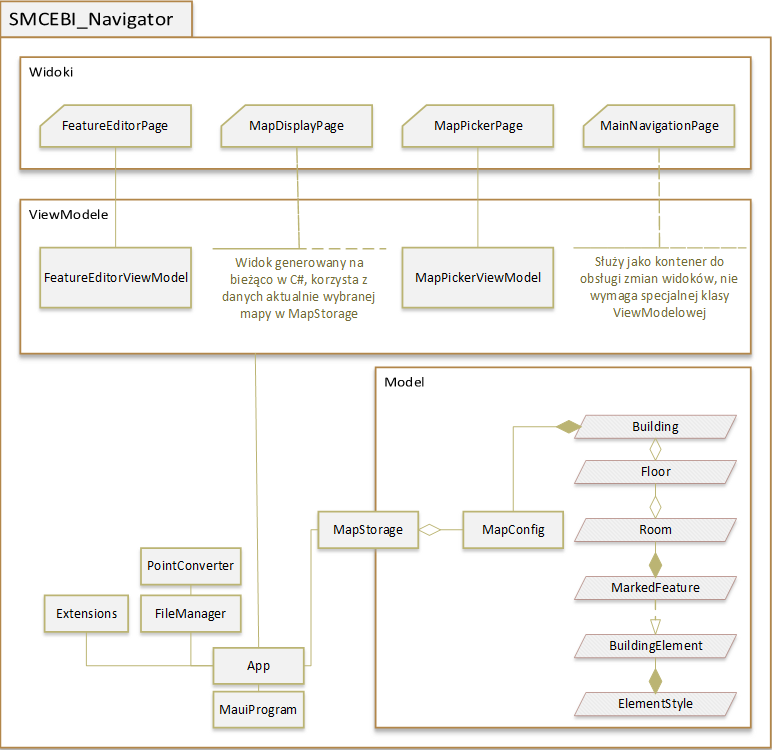
\includegraphics[width=0.99\textwidth]{shortClassDiagram.png}
    \caption{Diagram najważniejszych klas w projekcie SMCEBI Navigator}
    \label{img:shortClassDiagram}
\end{figure}
\newpage


Zgodnie z rysunkiem \ref{img:projectDiagram}, oprócz bezpośredniego kodu aplikacji, 
zdecydowałem się na wyodrębnienie 3 projektów:

\paragraph{NavigatorTests}
Projekt służący do statycznej analizy kodu poprzez przeprowadzenie testów jednostkowych.
Nie jest on obszerny, ale wraz z rozwojem oprogramowania może znaleźć się w nim więcej 
scenariuszy. Na potrzeby tej pracy został zaimplementowany jeden test pokazowy, 
żeby móc skonfigurować ich wywołanie za pomocą pipeline'a.

\paragraph{MapBuilder\_API\_Base}
Projekt definiuje interfejs \verb|IMapBuilder|, który należy zaimplementować przy dodawaniu 
do aplikacji biblioteki wyświetlającej mapę, tak jak stało się to w przypadku LeafletAPI.
Ten podział wprowadza kompatybilność i możliwość zmian minimalnym kosztem programistycznym.

W obecnej wersji dodanie biblioteki wymaga dodania projektu do rozwiązania, specjalnej opcji w enumeratorze 
\verb|MapEngine| oraz dodanie odpowiedniej metody do \verb|ConfigParser|. Wraz z rozwojem aplikacji 
planuję ten proces skrócić do dołączenia biblioteki poprzez mechanizm refleksji~\cprotect\footnote{%
    Specjalna biblioteka \verb|System.Reflection| pozwala na dynamiczne włączanie do programu 
    dodatkowych bibliotek \verb|.dll| w trakcie uruchomienia aplikacji, co pozwala na rozbudowanie 
    funkcji programu. Taki system może być skomplikowany oraz niebezpieczny, więc zdecydowałem się 
    na odsunięcie tej decyzji w czasie.
}.

\paragraph{LeafletAPI}
W projekcie zaimplementowałem generowanie strony HTML z wykorzystaniem wspomnianej biblioteki Leaflet~\cite{leafletGithub}.
Biblioteka tworzy obiekt \verb|MapBuilder| implementujący interfejs \verb|IMapBuilder|, który jest 
za pomocą aplikacji poszerzany o kolejne piętra, pokoje oraz obiekty z kreatora, a po wywołaniu 
metody \verb|Build| zwraca wynikowy skrypt, który zostaje zwrócony do aplikacji.

W zrozumieniu działania biblioteki, nieopisaną pomocą okazał się projekt Floorplans~\cite{floorplansGithub},
na którego podstawie byłem w stanie wstępnie sprawdzić zachowanie przeglądarkowych kontrolek, 
a następnie za pomocą inżynierii wstecznej zaimplementować jego funkcjonalność w uniwersalny sposób.


